\documentclass{llncs}

\usepackage{times,graphicx,epsfig,boxedminipage,url,xspace,array,amsmath,textcomp}

\begin{document}

\thispagestyle{empty}
\title{Formal Verification of Real-Time Data Processing of the LHC Beam Loss Monitoring System: A Case Study}
\author{Naghmeh Ghafari \inst{1} \and Ramana Kumar \inst{2} \and Jeff Joyce \inst{1}
  \and Bernd Dehning \inst{3} \and Christos Zamantzas \inst{3} }
\institute{Critical Systems Labs, Vancouver, BC, Canada
  \and University of Cambridge, Cambridge, UK
  \and CERN, Geneva, Switzerland}

\pagestyle{plain}

\maketitle

\begin{abstract}

We describe a collaborative effort in which the HOL4 theorem prover is being used to formally verify properties of a structure within the Large Hadron Collider (LHC) machine protection system at the European Organization for Nuclear Research (CERN).
This structure, known as \emph{Successive Running Sums} (SRS), generates the primary input to the decision logic that must initiate a critical action by the LHC machine protection system in response to the detection of a dangerous level of beam particle loss.
The use of mechanized logical deduction complements an intensive study of the SRS structure using simulation.
We are especially interested in using logical deduction to obtain a generic result that will be applicable to variants of the SRS structure.
This collaborative effort has individuals with diverse backgrounds ranging from theoretical physics to system safety.
The use of a formal method has compelled the stakeholders to clarify intricate details of the SRS structure and behaviour.
\end{abstract}

\section{Introduction}

The Large Hadron Collider (LHC) at the European Organization for Nuclear Research (CERN) is a high-energy particle accelerator.
It is designed to provide head-on collisions of protons at a center of a mass energy of 14 TeV for high-energy particle physics research.
In order to reach the required magnetic field strengths, the LHC has superconducting magnets cooled with superfluid helium.
Due to the high energy stored in the circulating beams (700 MJ), if even a small fraction of the beam particles deposit their energy in the equipment, they can cause the superconductors to transition to their normal conducting state.
Such a transition is called a \emph{quench}.
The consequences of a quench range from several hours of downtime (for cooling the magnets down to their superconducting state), to months of repairs (in the case of equipment damage).

The main strategy for protecting the LHC is based on the Beam Loss Monitoring System (BLMS), which triggers the safe extraction of the beams if particle loss exceeds thresholds that are likely to result in a quench.
At each cycle of the two counter-rotating beams around the 27 km tunnel of LHC, the BLMS records and processes several thousands of data points to decide whether the beams should be permitted to continue circulating or whether their safe extraction should be triggered.
The processing includes analysis of the loss pattern over time and of the energy of the beam.

The BLMS must respond to dangerous losses quickly, but determining whether losses are dangerous may require analysis of loss data recorded over a long period of time.
Furthermore, the BLMS must continue recording large amounts of data in real-time while processing.
To achieve these goals, the BLMS maintains approximate cumulative sums of particle losses over a variety of sizes of moving windows.
The component responsible for maintaining these sums is called \emph{Successive Running Sums} (SRS).
The SRS component is implemented in hardware, in order to be fast enough to work in real-time, and on Field Programmable Gate Arrays (FPGAs) in particular so that they can be easily reprogrammed with future upgrades~\cite{Chris-FPGA}.

The SRS component has a complex structure and the correctness of its behaviour is critical for safe and productive use of the LHC.
Any error in the SRS implementation would either compromise the availability of the LHC (unnecessary request for beam dump) or safety (not triggering a necessary beam dump).
The current approach for analyzing the SRS implementation relies on the simulation of its behavior on sample streams of input for different loss scenarios~\cite{Chris-thesis}.

In this paper, we describe a formal verification approach based on logical deduction for analyzing the SRS implementation.
Our high level proof strategy takes advantage of the regular structure of the SRS, which consists of multiple layers of shift registers and some simple arithmetic hardware.
There is a degree of regularity in how the output of each layer is used as input to the next layer.
There is also a degree of regularity in the timing of each layer with respect to its position in the stack of layers.
This regularity serves as a basis for inductive reasoning, which makes the amount of verification effort impervious to the number of layers in the structure.

Compared to test-based methods, like simulation, formal methods not only offer much higher confidence in the correctness of a system's behavior, but also help improve our understanding of its specification.
One of the challenges in pursuing a formal verification approach for SRS was capturing the intricate details of the system's specification via experiment and refinement with a team of different backgrounds and expertise.
Our confidence in the SRS design as a result of this effort ultimately rests upon our deep understanding of why the design is correct rather than the fact that we obtained ``Theorem Proved" as the final output of a software tool.
In particular, our use of mechanized logical deduction was a highly iterative process that incrementally refined our understanding of (1) the implementation (2) the intended behavior and (3) the ``white board level" argument or explanation for why the implementation achieves the intended behaviors.
The most important use of HOL4  was its role as an ``implacable skeptic" that compelled us to really understand the details~\cite{rushby}.

Our contributions in this paper are: a formal model of the SRS component of the BLMS, a formal analysis of its behavior, and commentary on the process and outcomes of taking a formal approach.
We give an overview of the BLMS in Section~\ref{sec-BLM}, and describe the SRS component in particular in Section~\ref{sec-SRS}.
In Section~\ref{sec-verification}, we describe our approach to formal verification, and present the formal model and results.
Finally, we reflect on the process, summarising lessons learned and future directions, in Section~\ref{sec-conclusions}.

\section{BLMS Overview}
\label{sec-BLM}

\begin{figure}[t]
  \centering  \scalebox{0.7}{ 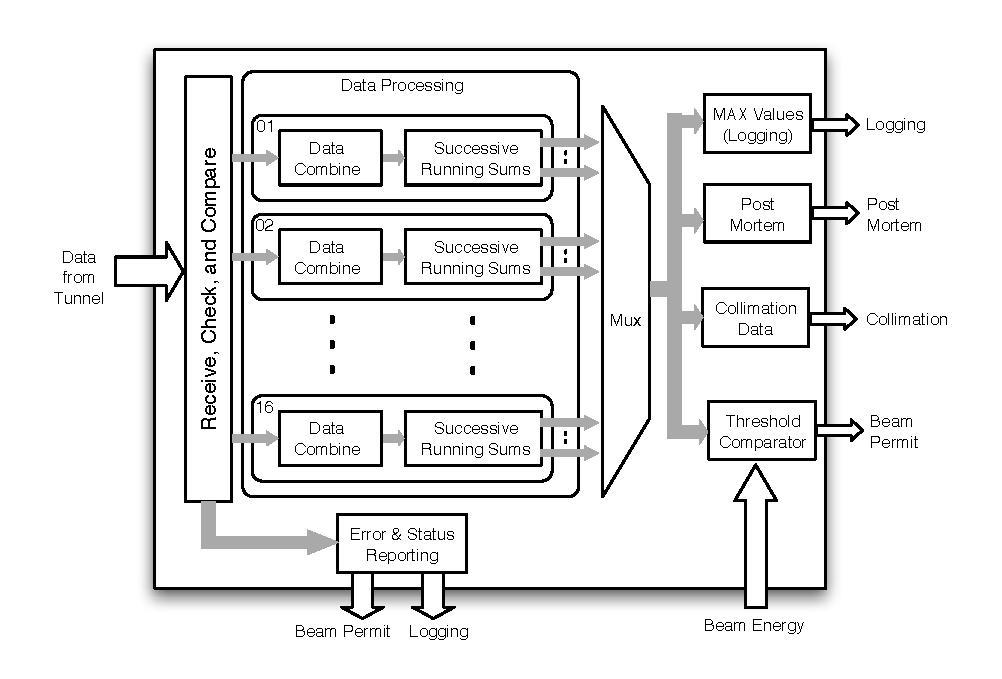
\includegraphics{BLETC.eps}}
   \caption{Block diagram of a BLETC card.}
  \label{fig:BLETC}
\end{figure}

The main purpose of the BLMS is to measure particle loss, and to request beam extraction if the loss level indicates that a quench is likely to occur.
The physical principle underlying particle loss measurement \cite{Dehning-IPAC,Chris-FPGA} is the detection of energy deposited by \emph{secondary shower particles} using specially-designed detectors called  \emph{ionization chambers}.
There are approximately 4000 ionization chambers strategically placed on the sides of the magnets all around the LHC tunnel underground.
The ionization chambers produce electrical signals, based on the recording of shower particles, which are read out by \emph{acquisition cards}.
Acquisition cards, also located in the tunnel and therefore implemented by radiation-tolerant electronics, acquire and digitize the data and transmit the digitized data to the surface above the tunnel using optical links.
At the surface, data processing cards named \emph{BLETCs} receive the data and decide whether or not the beam should be permitted to be injected or to continue circulating.
Each acquisition card receives data from eight ionization chambers, and each BLETC receives data from two acquisition cards.
A BLETC provides data to the Logging, Post Mortem, and Collimation systems that drive on-line displays in the control room, perform long-term storage for offline analysis, and setup the collimators automatically.
Due to demanding performance requirements, BLETCs are implemented on FPGAs, which include the resources needed to implement complex processing and can be reprogrammed making them ideal for future upgrades or system specification changes.

Figure~\ref{fig:BLETC} shows a block diagram of the processes on a BLETC FPGA.
In the following, we briefly describe each of the four processing blocks on a BLETC card.

\emph{(a) Receive, Check, and Compare (RCC)}: The RCC block receives the data directly from the acquisition card, and attempts to detect and correct erroneous transmissions by using Cyclic Redundancy Check and 8B/10B algorithms~\cite{CRC,8B10B}.

\emph{(b) Data Processing}: Whether or not a quench results from particle loss depends on the loss duration and the beam energy.
Given the tolerance acceptable for quench prevention, the quench threshold versus loss duration is approximated by the minimum number of sliding integration windows (called \emph{Running Sums}) fulfilling the tolerance.
In order to achieve the \emph{dynamic range} (domain of variation of losses) required by the specification, the detectors use both Current-to-Frequency converter and Analogue to Digital convertor circuitries.
The data processing block merges these two types of data coming from a detector so as to send a single count value to the SRS block.
The implementation of the SRS block is described in Section~\ref{sec-SRS}.

\emph{(c) Threshold Comparator}: Every running sum needs to be compared to the threshold that was chosen by the beam energy reading at that moment.
The comparator initiates a beam dump request if any of the running sums is higher than its corresponding threshold.
Beam dump requests are forwarded to the Beam Interlock System which initiates the beam dump.
There are 12 running sums calculated for each 16-detector channel allocated to a BLETC card.
The beam energy information is scaled to 32 levels (0.45 to 7 TeV) and each processing module holds data only for those 16 connected detectors.
Thus, a total of 6,144 threshold values need to be held on each card.

\emph{(d) Logging, Post Mortem and Collimation}:  To be able to trace back the loss signal development, the BLMS stores the loss measurement data.
This data is sent to Logging and Post-Mortem systems for online viewing and storage.
For the purpose of supervision, the BLMS drives an online event display to show error and status information recorded by the tunnel electronics and the RCC process as well as the maximum loss rates seen by the running sums.
Each BLETC card also provides data to the Collimation system for the correct alignment and setup of the collimators.

\section{Successive Running Sums (SRS)}
\label{sec-SRS}

\begin{figure}[t]
  \centering 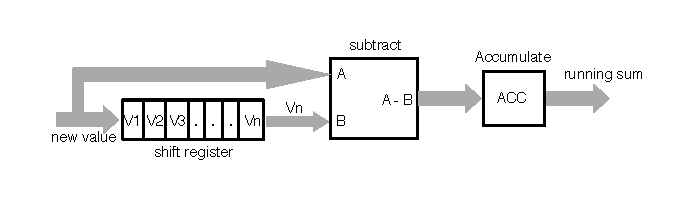
\includegraphics{rs.eps}
   \caption{Block diagram showing how to produce and maintain a continuous running sum of arriving values.}
  \label{fig:RS-basic}
\end{figure}

Beam losses can happen at different rates, compared to the number of cycles of the beam around the tunnel.
One-cycle failures are called \emph{ultra-fast} losses.
Multi-cycle losses can be classified as: \emph{very fast} losses, which happen in less than 10 ms; \emph{fast} losses, which happen between 10 ms and 1 s; and, \emph{steady} losses, where the beam is lost over one second or more~\cite{Schmidt-ICFA}.

Processing the data collected by the detectors, referred to as \emph{count} values, involves an analysis of the loss pattern over time, accounting for the energy of the beam.
The processing procedure is based on the idea that a constantly updated moving window can be maintained in an accumulator by adding the incoming (newest) value and subtracting the oldest value (see Figure~\ref{fig:RS-basic}).
The number of values in the window is its \emph{integration time}.
Ideally, we would have an unbounded number of windows with lengths covering the whole spectrum of times from 40 micro-seconds (the rate at which count values enter a BLETC card) to 100 seconds, for detecting all losses from ultra-fast up to steady.
To approximate this ideal with finite resources, the BLMS is given the tolerance acceptable for quench prevention, and the quench threshold versus loss duration curve is approximated by the minimum number of windows that meet the tolerance.

\begin{figure}[t]
  \centering 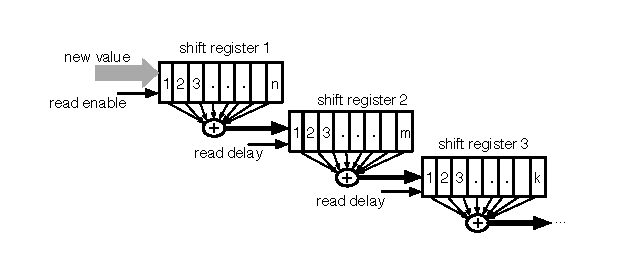
\includegraphics{SRS-basic.eps}
   \caption{Block diagram showing a configuration for efficient summation of many values.}
  \label{fig:SRS-basic}
\end{figure}

Long moving windows, that is, windows with large integration times, are required, which means keeping long histories of received count values.
To accomplish this goal with relatively narrow shift registers, the SRS uses consecutive storage of sums of counts.
Instead of storing all the values needed for a sum, the SRS accumulates many values as a partial sum, thereby using only a fraction of the otherwise needed memory space.
The partial sums for a window with a large integration time are chosen so that they also serve as the sums calculated by a window with a smaller intergration time.
This technique works by feeding the sum of one shift register's contents, every time its contents become completely updated, to the input of another shift register (see Figure~\ref{fig:SRS-basic}).
By cascading shift registers like this, very long moving windows can be constructed using a significantly small amount of memory.
This scheme is the basis for the SRS implementation in each BLETC.

The SRS implementation minimizes resource usage by using smaller, previously calculated, running sums in the calculation of larger, later running sums, which therefore do not need extra summation values to be stored.
In addition, it makes use of multipoint shift registers that are configured to give intermediate outputs, referred to as \emph{taps}.
The taps provide data outputs at certain points in the shift register chain, thus contributing to the efficient use of resources.

In the SRS implementation, one shift register's sum is fed as input to another shift register.
Therefore, the best achievable latency of each shift register is equal to the refreshing time of its preceding shift register, i.e., the time needed to completely update its contents.
The \emph{read delay} signal (see Figure~\ref{fig:SRS-basic}) of each shift register holds a delay equal to this latency to ensure correct operation.
The delay is equal to the preceding shift register's delay multiplied by the number of cells to be used in the sum.

\begin{figure}[t]
  \centering \scalebox{0.65}{ 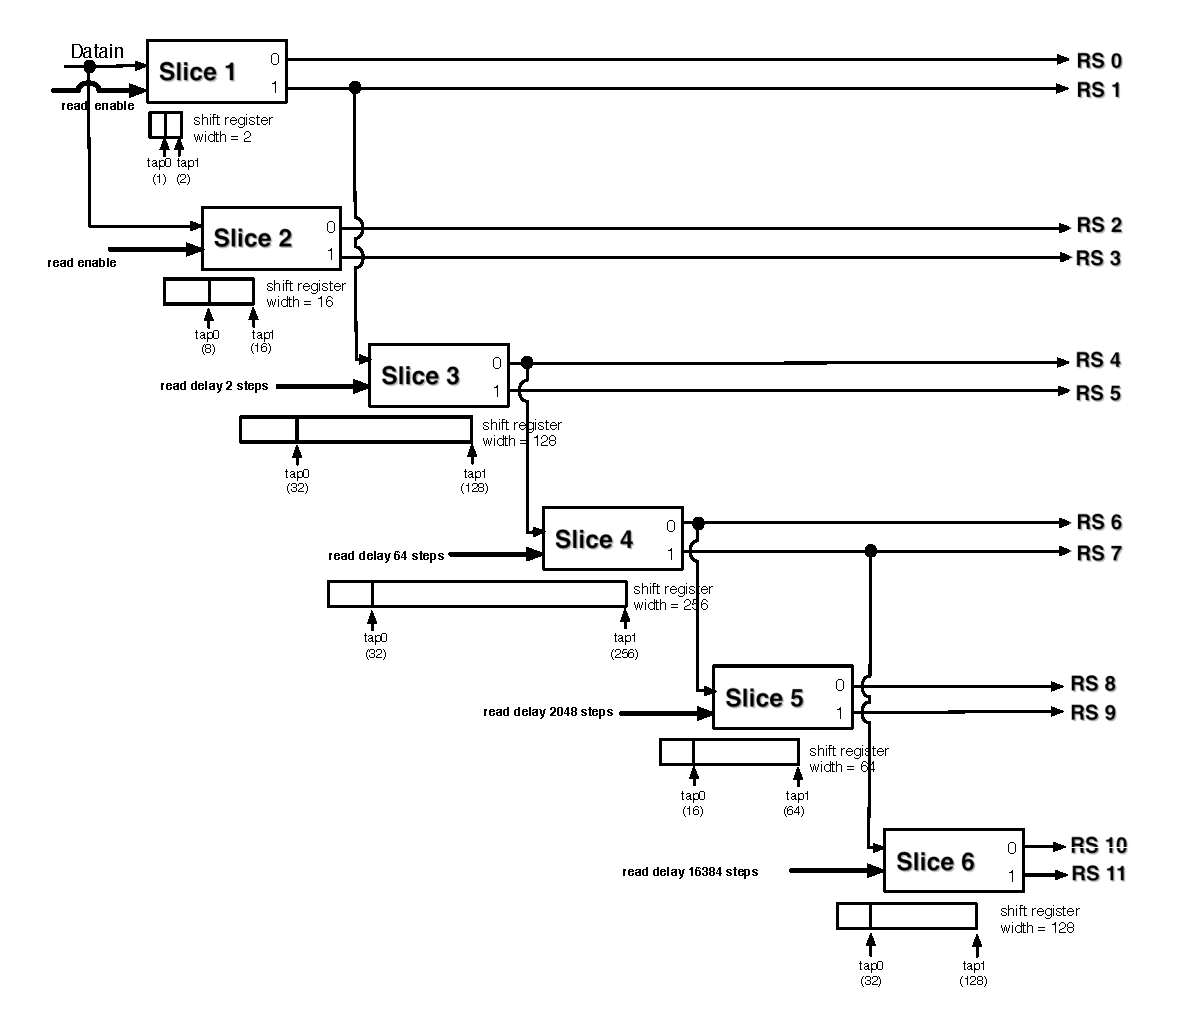
\includegraphics{srs-modified.eps}}
   \caption{Block diagram showing the implementation of SRS in a BLETC.}
  \label{fig:srs}
\end{figure}

Figure~\ref{fig:srs} shows the implementation of SRS in a BLETC.
It consists of 6 \emph{slices}, where each slice computes two running sums (e.g., slice 4 computes the fourth and fifth running sums: RS6 and RS7) with the use of a multipoint shift register, two subtractors and two accumulators (see Figure~\ref{fig:slice}).

As shown in Table~\ref{fig:SRS-table}, cascading 6 slices is enough to reach the 100 second integration limit required by the specifications given by the scientists and engineers who designed the machine protection strategy for the LHC.

\begin{figure}[t]
  \centering \scalebox{0.8}{ 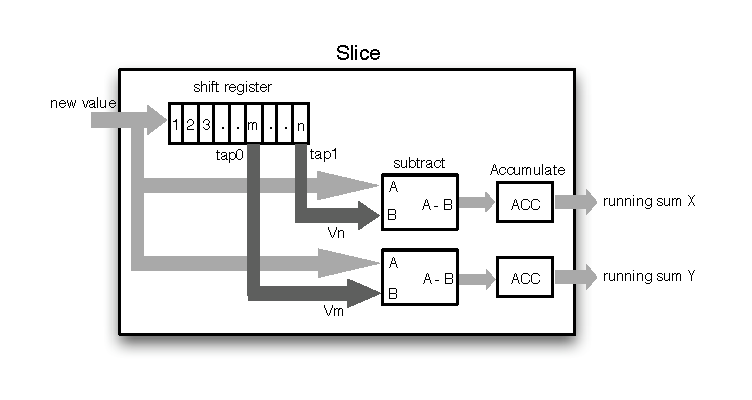
\includegraphics{multi-rs.eps}}
  \vspace{-0.1in}
   \caption{Block diagram showing the implementation of each slice.}
  \label{fig:slice}
\end{figure}

\begin{table}[t]
\centering
\begin{tabular}{|r|r|r|r|c|l|}
\hline
\multicolumn{2}{|c}{Range} &\multicolumn{2}{|c|}{Refreshing} & & \\\cline{1-4}
40 {\textmu}s steps & ms & 40 {\textmu}s steps  & ms & slice & running sum \\\hline\hline
1 & 0.04 & 1 & 0.04 & slice 1 & RS0 \\\hline
2 & 0.08 & 1 & 0.04 & slice 1 & RS1 \\\hline
8 & 0.32 & 1 & 0.04 & slice 2 & RS2 \\\hline
16 & 0.64 & 1 & 0.04 & slice 2 & RS3 \\\hline
64 & 2.56 & 2 & 0.08 & slice 3 & RS4 \\\hline
256 & 10.24 & 2 & 0.08 & slice 3 & RS5 \\\hline
2048 & 81.92 & 64 & 2.56 &slice 4 & RS6 \\\hline
16384 & 655.36 & 64 & 2.56 &slice 4 & RS7 \\\hline
32768 &1310.72 & 2048 & 81.92 & slice 5 & RS8 \\\hline
131072 & 5242.88 & 2048 & 81.92 & slice 5 & RS9 \\\hline
524288 & 2097.52 & 16384 & 655.36 & slice 6 &RS10 \\\hline
2097152 & 83886.08 & 16384 & 655.36 & slice 6 & RS11 \\\hline
\end{tabular}
\vspace{2ex}
\caption{SRS configuration in BLETC.}
\label{fig:SRS-table}
\end{table}

\section{Verification of the SRS Implementation using HOL4}
\label{sec-verification}

\subsection{Introduction}
Our formal verification effort uses mechanised logical deduction, or \emph{theorem proving}.
In general, theorem proving is used to show that desired properties of a system are logically implied by a formal model of the system.
We use the HOL4 open source software tool~\cite{HOL4,DBLP:conf/tphol/SlindN08}, which was developed initially at the University of Cambridge, but now by an international team.
HOL4 enables the construction of theories in Higher-Order Logic (HOL)~\cite{DBLP:journals/jsyml/Church40}, a formal logic with a similar expressive power to set theory that is widely used for formalising hardware and software models and statements about them.
The implementation of HOL4 uses Milner's LCF approach~\cite{Milner:1972:LCF:891954}: a small ``kernel'' implementing the primitive rules of the logic, and convenient derived rules and tactics implemented in terms of the kernel.
Every theorem ultimately comes from the kernel, and this fact provides high assurance of the logical soundness of the verification results obtained using the system.

HOL4 is an \emph{interactive} theorem prover: the user provides the high level proof strategy by composing functions that automate common chains of logical deduction.
The work described here could have been done using other systems such as HOL Light~\cite{HOLLight,DBLP:conf/tphol/Harrison09a}, Isabelle/HOL~\cite{Isabelle}, ProofPower~\cite{ProofPower}, PVS~\cite{PVS,DBLP:conf/tphol/OwreS08} or Coq~\cite{Coq}.
The first three use essentially the same higher-order logic as HOL4, whilst PVS and Coq support more powerful logics.
%<What about ACL2?>
While offering less ``push-button'' automation than other kinds of formal verification such as model-checking, machine-assisted theorem proving is appropriate for verifying the SRS, since it is unlikely that the correctness theorems, which need lemmas proved by manually guided mathematical induction, could be generated automatically.

Our goal is to build a generic model of the SRS structure, and to prove that it satisfies its specification, that it calculates approximate running sums of received count values within acceptable error margins.
Let $\mathsf{RS}\;n$ denote, as in Figure~\ref{fig:srs}, the $n$-th output of the SRS structure, which is supposed to compute a sum of received count values, and let $\mathsf{true\_sum}\;n$ denote this sum.
The multi-layered structure of the SRS and the read delay of each shift register result in the outputs of SRS being delayed from the $\mathsf{true\_sum}$ values.
A sketch of the desired correctness statement is: \[\forall{n} \cdot \, \mathsf{RS}\;n= \mathsf{true\_sum}\; n \pm\text{acceptable error}\]
Although Figure~\ref{fig:srs} suggests that the SRS structure has only twelve outputs  (i.e. $0\leq{n}\leq11$), we obtain a more generic result (that is useful in future upgrades of the system) by proving the correctness of the above statement for all values of $n$.

To make the above correctness statement more precise, we need to include the notion of time.
The count values arrive at the input of the SRS block every 40 micro-seconds, which we abstract as a single time step in our logical model.
We formalize the input stream as a function of time: $D\;t$ denotes the input value to the SRS structure at time $t$.
In addition, the terms in the above statement depend on this stream of input counts.
With these refinements, the correctness statement becomes: \[\forall{D\,n\,t} \cdot \,\mathsf{RS}\;D\;n\;t = \mathsf{true\_sum}\;D\;n\;t\pm\text{acceptable error}\]

\subsection{Formal Model of SRS}
The first step to prove the correctness statement is to build a logical model of the SRS structure.
We model each building block of the SRS structure that holds a count value -- for example, each cell in each shift register -- as a function in HOL\footnote{The acronym HOL refers to higher-order logic rather than the software tool HOL4.
We use the tool to define a function in the logic.}

Our model is both a simplification and a generalization of the actual structure of SRS in BLMS in the following sense.
We model an infinite number of slices (rather than six slices), each with an infinite number of shift register cells and taps (rather than fixed width shift registers and only two taps), simply by letting indices range over the natural numbers without explicitly giving limits.
This parameterization makes the model more likely to be applicable to future versions of the system, but also fits more naturally into HOL than would a finite model.
We defined our formal model to be at a level of abstraction above the details of circuity that implements basic arithmetic operations.
We use natural numbers throughout, rather than, for example, finite words that would more accurately model count values.
This level of abstraction is sufficient for the SRS correctness properties we are interested in.
A separate verification effort can focus on showing that a more realistic model of hardware circuitry accurately implements natural number arithmetic.


\begin{table}[t]
\begin{tabular}{lp{0.8\textwidth}}
Function&Intended meaning\\
\hline
\(\mathsf{tap}\;n\;x\)&The position of tap $x$ of slice $n$. (The first position is $0$.)\\
\(\mathsf{input}\;n\)&A pair $(n',x)$ indicating that the input to slice $n$ is output $x$ of slice $n'$.\\
\(\mathsf{delay}\;n\)&The number of time steps between updates of slice $n$.\\
\(\mathsf{source}\;D\;n\;m\;t\)&The value of the cell that is the direct input to cell $m$ of slice $n$, at time $t$, given input stream $D$.\\
\(\mathsf{SR}\;D\;n\;m\;t\)&The value of cell $m$ of shift register $n$, at time $t$, given input stream $D$.\\
\(\mathsf{output}\;D\;n\;x\;t\)&The output at tap $x$ of slice $n$, at time $t$, given input stream $D$.\\
\(\mathsf{RS}\;D\;n\;t\)&The $n$-th running sum at time $t$, given input stream $D$.\\
\(\mathsf{update\_time}\;n\;t\)&A boolean indicating whether $t$ is an update time for slice $n$.
\end{tabular}
\vspace{2ex}
\caption{
Descriptions of the HOL functions comprising our model of the SRS structure.
\label{tab:descriptions}
}
\end{table}

Table~\ref{tab:descriptions} lists the HOL functions comprising our model along with their intended meanings.
The arrangement of the slices is described by functions $\mathsf{input}\;n$ and $\mathsf{tap}\;n\;x$.
The read delay of a slice is modeled by $\mathsf{delay}\;n$.
Each slice is modeled by three functions: $\mathsf{SR}\;D\;n\;m\;t$ represents the value of each cell of the slice's shift register, $\mathsf{source}\;D\;n\;m\;t$ represents the direct input of each cell, and $\mathsf{output}\;D\;n\;x\;t$ represents the value of the slice's output at its taps.
The function $\mathsf{RS}\;D\;n\;t$ models the running sums and $\mathsf{update\_time}\;n\;t$ checks if it is time to refresh the contents of a slice.
We have both $\mathsf{RS}$ and $\mathsf{output}$ functions, though $\mathsf{RS}$ is easily defined in terms of $\mathsf{output}$, because $\mathsf{RS}$ represents an SRS output (indexed by a single number), whereas $\mathsf{output}$ represents an individual slice output (indexed by slice and tap numbers).
By separating $\mathsf{RS}$ and $\mathsf{output}$, we allow for designs where some slice outputs are not SRS outputs, but may still be used internally as inputs to other slices.

The formal definitions of the functions listed in Table~\ref{tab:descriptions} are given in Figure~\ref{fig:definitions}.
Note that the definition of $\mathsf{input}$ when $n=0$ or when $n>6$ does not change the structure presented.
A similar comment applies to other definitions when $n$, representing a slice number, is $0$, or when $x$, representing a shift register position, is greater than $1$.
We define all excess taps (where $x > 1$) to be in the same position as the last tap.

%Some text description for Figure 7, we can remove it later on
As explained in Section~\ref{sec-SRS}, the delay of each slice is equal to the delay of the slice it receives its input from multiplied by the number of the elements in the input slice used for the sum.
For example in Figure~\ref{fig:srs}, $\mathsf{delay}\;4 = \mathsf{delay}\;3 \times \mathsf{tap}\;3\;0 = 2 \times 32$.
The definition of the $\mathsf{source}$ function states that the source of each cell $m$ in a shift register is cell $m-1$, except for the first cell whose source is the output of the input slice.
For example, $\mathsf{source}\;D\;4\;7\;t = \mathsf{SR}\;D\;4\;6\;t$ and $\mathsf{source}\;D\;4\;0\;t = \mathsf{output}\;D\;3\;0\;t$.
The output of each slice is computed every time the contents of its shift register are updated by adding the incoming newest value (specified by $\mathsf{source}$) and subtracting its oldest value, that is the value in the cell at the tap position.
The content of each cell of a shift register, $\mathsf{SR}\;D\;n\;m\;t$  is also computed at every update time based on the value of its source.
Every definition in Figure~\ref{fig:definitions} is \emph{local} (only represents a small part of the SRS structure) and therefore verification against its intended meaning is relatively straightforward.

Figure~\ref{fig:auxdefs} shows the definition of a set of additional functions required to prove our main results.
The function $\mathsf{delay\_sum}\;n$ represents the cumulative delay of the preceding shift registers of a slice.
For example, $\mathsf{delay\_sum}\;4 = \mathsf{delay}\;3 + \mathsf{delay}\;1 + \mathsf{delay}\;0 = 2 +1 +1 = 4$.
The function $\mathsf{last\_update}\;n\;t$ specifies the time that the $n$-th slice last updated, and $\mathsf{exact}\;D\;n\;x\;t$ computes the exact sum of consecutive input counts, without delay, that $\mathsf{output}\;D\;n\;x\;t$ is supposed to approximate.


\begin{figure}[t]
\begin{tabular}{ll}
$\;\mathsf{tap}\;0\;0=0\quad\quad$ & $\mathsf{tap}\;0\;x=0$\\
$\;\mathsf{tap}\;1\;0=1-1\quad$ &  $\mathsf{tap}\;1\;x=2-1$\\
$\;\mathsf{tap}\;2\;0=8-1\quad$ &  $\mathsf{tap}\;2\;x=16-1$\\
$\;\dots\quad$ & $\mathsf{tap}\;6\;x=128-1\quad\text{(where each $x>0$)}$\\[1ex]

$\;\mathsf{input}\;0=(0,0)\quad$ & $\mathsf{input}\;1=(0,0)$\\
$\;\mathsf{input}\;2=(0,0)\quad$ & $\mathsf{input}\;3=(1,1)$\\
$\;\mathsf{input}\;4=(3,0)\quad$ & $\mathsf{input}\;5=(4,0)$\\
$\;\mathsf{input}\;6=(4,1)\quad$ & $\mathsf{input}\;n=(n-1,0)\quad\text{(where $n>6$)}$\\[1ex]

$\;\mathsf{delay}\;0=1$\\
\multicolumn{2}{l}{$\;\mathsf{delay}\;n=\mathsf{delay}\;n'\times((\mathsf{tap}\;n'\;x)+1)$}\\
\multicolumn{2}{l}{$\qquad\qquad\qquad\text{where $(n',x)=\mathsf{input\;n}$ (and $n>0$)}$}\\[1ex]

\multicolumn{2}{l}{\;$\mathsf{source}\;D\;n\;0\;t=\mathsf{output}\;D\;n'\;x\;t\quad\text{where $(n',x)=\mathsf{input\;n}$}$}\\
\multicolumn{2}{l}{$\;\mathsf{source}\;D\;n\;m\;t=\;\mathsf{SR}\;D\;n\;(m-1)\;\quad\text{(where $m>0$)}$}\\[1ex]

\multicolumn{2}{l}{\;$\mathsf{SR}\;D\;n\;m\;0=0$}\\
\multicolumn{2}{l}{$\;\mathsf{SR}\;D\;n\;m\;t=\text{if $\mathsf{update\_time}\;n\;t$ then }$}\\
&$\mathsf{source}\;D\;n\;m\;(t-1)$\\
\multicolumn{2}{l}{$\qquad\qquad\qquad\quad\text{else }\mathsf{SR}\;D\;n\;m\;t\qquad\text{(where $t>0$)}$}\\[1ex]

\multicolumn{2}{l}{$\;\mathsf{output}\;D\;0\;x\;t=D\;t$}\\
\multicolumn{2}{l}{$\;\mathsf{output}\;D\;n\;x\;0=0$}\\
\multicolumn{2}{l}{$\;\mathsf{output}\;D\;n\;x\;t = \text{if $\mathsf{update\_time}\;n\;t$ then }$}\\
\multicolumn{2}{l}{$\qquad\quad((\mathsf{output}\;D\;n\;x\;(t-1))+(\mathsf{source}\;D\;n\;0\;(t-1)))-{}$}\\
&$\qquad\qquad\qquad(\mathsf{SR}\;D\;n\;(\mathsf{tap}\;n\;x)\;(t-1))$\\
\multicolumn{2}{l}{$\qquad\qquad\qquad\qquad\text{else }\mathsf{output}\;D\;n\;x\;(t-1)\qquad\text{(where $n,t>0$)}$}\\[1ex]

\multicolumn{2}{l}{$\;\mathsf{RS}\;D\;n\;t=\mathsf{output}\;D\;\left(\left\lfloor\frac{n}{2}\right\rfloor+1\right)\;(n\operatorname{mod}2)$}\\[1ex]

\multicolumn{2}{l}{$\;\mathsf{update\_time}\;n\;t\iff(t\operatorname{mod}\mathsf{delay}\;n=0)$}
\end{tabular}
\vspace{2ex}
\caption{
\label{fig:definitions}
Definitions of the HOL functions comprising our model of the SRS structure.
\(\mathsf{tap}\) and \(\mathsf{input}\) are defined to match Figure~\ref{fig:srs}.
Slice $0$ is a virtual slice representing the SRS input; this enables a succinct definition of $\mathsf{source}$.}
\end{figure}

\begin{figure}[t]
\begin{tabular}{l}
$\mathsf{delay\_sum}\;0=0$\\
$\mathsf{delay\_sum}\;n=\mathsf{delay}\;n'+\mathsf{delay\_sum}\;n'\quad\text{where $(n',\_)=\mathsf{input}\;n$}$\\[1ex]

$\mathsf{last\_update}\;n\;0=0$\\
$\mathsf{last\_update}\;n\;t=\text{if $\mathsf{update\_time}\;n\;t$ then $t$}$\\
$\quad\;\;\qquad\qquad\qquad\text{else }\mathsf{last\_update}\;n\;(t-1)\quad\text{(where $t>0$)}$\\[1ex]

$\mathsf{exact}\;D\;n\;x\;t=\displaystyle\sum_{m=0}^{((\mathsf{tap}\;n\;x)+1)\times(\mathsf{delay}\;n)}\begin{cases}0&t<m+1\\D\;(t-m-1)&\text{otherwise}\end{cases}$
\end{tabular}
\vspace{2ex}
\caption{
\label{fig:auxdefs}
Definitions of auxiliary HOL functions used while proving theorems about the model of the SRS structure.}
\end{figure}



\subsection{Theorems about the Model}
Our central result equates the output of a slice to a sum of consecutive input counts.
More precisely, it says that if slice $n$ was just updated, then the output at tap $x$ is equal to the sum of $((\mathsf{tap}\;n\;x)+1)\times(\mathsf{delay}\;n)$ input values, starting from the input $\mathsf{delay\_sum}\;n$ time steps ago.

\begin{theorem}\label{output_input_at_update_times}
For all values of $D$, $n$, and $x$, the $\mathsf{output}$ of slice $n>0$ at an update time $t$ satisfies
\begin{equation*}
\mathsf{output}\;D\;n\;x\;t=\sum_{m=0}^{((\mathsf{tap}\;n\;x)+1)\times(\mathsf{delay}\;n)-1}\begin{cases}0 \qquad\qquad\qquad  t<m+\mathsf{delay\_sum}\;n\\D\;(t-m-\mathsf{delay\_sum}\;n)\quad\text{otherwise}\end{cases}
\end{equation*}
\end{theorem}

\begin{proof}
The shift register of slice $n$ is updated every $\mathsf{delay}\;n$ time steps.
When updated, the values in its cells are shifted one cell.
Therefore\footnote{For presentation convenience, here, we do not provide the details regarding the case when $t$ is small, for example $t<m\times\mathsf{delay}\;n$.
For complete theorem statements and the proof script, please refer to \url{https://github.com/xrchz/CERN-LHC-BLMTC-SRS/blob/master/hol/srsScript.sml}.},
\begin{equation*}
\mathsf{SR}\;D\;n\;(m+1)\;t=\mathsf{SR}\;D\;n\;m\;(t-\mathsf{delay}\;n)
\end{equation*}
By induction on $m$, using the above,
\begin{equation*}
\mathsf{SR}\;D\;n\;m\;t=\mathsf{SR}\;D\;n\;0\;(t-(m\times\mathsf{delay}\;n))
\end{equation*}
By induction on $t$, we can show that $\mathsf{output}\;D\;n\;x\;t$ is a sum of values of consecutive shift register cells
\begin{equation*}
\mathsf{output}\;D\;n\;x\;t=\sum_{m=0}^{\mathsf{tap}\;n\;x}\mathsf{SR}\;D\;n\;m\;t
\end{equation*}
Combining the last two results, $\mathsf{output}\;D\;n\;x\;t$ is a sum of consecutive values of the first shift register cell, $\mathsf{SR}\;D\;n\;0$.
Thus, we can express $\mathsf{output}\;D\;n\;x\;t$ in terms of $\mathsf{output}\;D\;n'\;x'\;t$, where $(n',x')=\mathsf{input}\;n$, since the source of $\mathsf{SR}\;D\;n\;0$ is the previous (input) slice's output.
Finally, by induction on $n$, we can express $\mathsf{output}\;D\;n\;x\;t$ as a function of $D$ alone, as required, using the result above for the inductive case.
\qed
\end{proof}

Since the outputs of a slice stay constant between update times for the slice, Theorem~\ref{output_input_at_update_times} suffices to characterize all outputs at all times.
Thus, the SRS structure's outputs are equal to the exact running sums of the input counts over windows whose sizes depend on the the width of the slice's shift register and position of the taps.
However, the sums are delayed by the total delay across all previous slices (represented by $\mathsf{delay\_sum}$).

The fact that the SRS calculates exact, but delayed, sums, is captured in the next theorem, which relates $\mathsf{output}\;D\;n\;x\;t$ to $\mathsf{exact}\;D\;n\;x$ at an earlier time.

\begin{theorem}\label{output_eq_exact}
For all values of $D$, $n$, and $x$, the $\mathsf{output}$ of slice $n>0$ at all times $t$ satisfies
\begin{equation*}
\mathsf{output}\;D\;n\;x\;t=\begin{cases}0\qquad\qquad\qquad\qquad\qquad\quad\mathsf{last\_update}\;n\;t+1<\mathsf{delay\_sum}\;n\\\mathsf{exact}\;D\;n\;x\;(\mathsf{last\_update}\;n\;t+1-\mathsf{delay\_sum}\;n)\quad\text{otherwise}\end{cases}
\end{equation*}
\end{theorem}
\begin{proof}
The proof follows from Theorem~\ref{output_input_at_update_times}, using the definition of $\mathsf{exact}$, and the fact that $\mathsf{output}\;D\;n\;x\;t$ has the same value as at the last update time.\qed
\end{proof}

The function $\mathsf{true\_sum}$ is easily defined in terms of $\mathsf{exact}$, namely, $\mathsf{true\_sum}\;D\;n\;t = \mathsf{exact}\;D\;\left(\left\lfloor\frac{n}{2}\right\rfloor+1\right)\;(n\operatorname{mod}2)\;t$.
Since $\mathsf{RS}$ is similarly defined in terms of the $\mathsf{output}$, Theorem~\ref{output_eq_exact} establishes a relationship between the values of $\mathsf{RS}$ and of $\mathsf{true\_sum}$.

We formulate the difference between the $\mathsf{RS}$ values and their corresponding $\mathsf{true\_sum}$s, caused by the delay, as $\mathsf{error}$.
To meet the tolerance acceptable for quench prevention, the SRS specification requires a bound on this $\mathsf{error}$.
Without restricting the input stream, the $\mathsf{error}$ is unbounded\footnote{For any bound, we can construct an input stream that causes the bound to be exceeded by, for example, having a sequence of zeroes followed by a sequence of count values much higher than the bound.}.
However, according to extensive experimental analysis, the beam loss over time follows some patterns.
By formulating some characterization of the input stream as constraints on $D$, we can recover a bound on the $\mathsf{error}$.
One of these constraints is a maximum value for the difference between two consecutive count values.
This ``maximum jump size'' can be inferred from the highest quench level thresholds.

Under such a constraint, we have proved a preliminary result bounding the error of $\mathsf{output}\;D\;n\;x\;t$ compared to $\mathsf{exact}\;D\;n\;x\;t$.
\begin{theorem}\label{max_error}
For all $k$ and $D$ satisfying $|D\;(t'+1)-D\;t'|\leq k$ at all times, the following holds for all slices $n>0$, tap positions $x$, and times $t$:
\begin{multline*}
t>(\mathsf{tap}\;n\;x+1)\times(\mathsf{delay}\;n)+\mathsf{delay}\;n+\mathsf{delay\_sum}\;n\implies\\
|\mathsf{output}\;D\;n\;x\;t-\mathsf{exact}\;D\;n\;x\;t|\leq(\mathsf{tap}\;n\;x+1)\times(\mathsf{delay\;n})\times k\times(\mathsf{delay}\;n+\mathsf{delay\_sum}\;n)
\end{multline*}
\end{theorem}
\begin{proof}
By applying Theorem~\ref{output_eq_exact}, we are left with an equation involving $\mathsf{exact}$ but not $\mathsf{output}$, specifically between $\mathsf{exact}\;D\;n\;x\;t$ and $\mathsf{exact}\;D\;n\;x\;(\mathsf{last\_update}\;n\;t+1-\mathsf{delay\_sum}\;n)$.
Our assumption on $t$ ensures that we are never in the $0$ case of either Theorem~\ref{output_eq_exact} or of the definition of $\mathsf{exact}$.
The function $\mathsf{exact}$ is defined as a sum of consecutive values of $D$, so we simply need to bound the difference between one such sum and another earlier one of the same size.
But if at each step the maximum difference is $k$, then the total difference is at most $k$ times the distance between the ends of the two sums, as required.
(We use the fact that $\mathsf{last\_update}\;n\;t=t-t\operatorname{mod}\mathsf{delay}\;n$ and, in general, that $a\operatorname{mod}b<b$.)
\end{proof}

The proof of Theorem~\ref{max_error} is straightforward when summarized, as above.
However, as for all of our theorems, there are several non-trivial details underlying the high-level summary provided.
For example, \emph{proving} that the maximum difference between the end terms in a sum is the maximum difference between consecutive elements multiplied by the number of terms requires an inductive argument.
Our HOL4 proof script for verification of SRS consists of 750 lines of code.
We proved 69 theorems, including 14 definitions.
In addition, we had to prove approximately 30 generic theorems that were added to HOL4 libraries during this work.

\section{Conclusions and Lessons Learned}
\label{sec-conclusions}

We described a case study in which the HOL4 theorem prover is used to formally verify properties of the SRS structure within the LHC machine protection system.
In this case study, we built a parameterized model of the SRS structure and showed that its behavior is correct with respect to its specification.
It is likely that the configuration of the slices and shift registers will need to change in the future as the understanding of the LHC and its weaknesses increases to accommodate more targeted protections
Thus, the parameterization in our model was crucial to make it applicable to the future upgrades.

One of our main challenges in this effort was building the formal model and formulating the correctness statements.
To understand the structure of the SRS, we started with a model of a simplified structure, which had a more regular arrangements of the slices and ignored the middle taps, and proceeded to a model which is closer to the SRS implementation in BLMS.
In addition, we used a basic spreadsheet simulation model for a few slices for sanity testing the correctness formulae.
However, some sanity tests related to Theorem 1 led us astray when we did not know the correct formula for that theorem.
The formulae we conjectured worked for small values of $n$, and simulating large values of $n$ was expensive, but the counterexamples were only on large values of $n$.
The most important use of mechanized logical deduction in this effort was its role as an ``implacable skeptic" that insisted we provide justification and compelled us to clarify the intricate details of the SRS structure and behavior.

The use of mechanized theorem proving to verify the correctness of the SRS behavior complements an intensive verification effort based on simulation performed at CERN.
This effort targeted the validity of the SRS as an accurate and fast enough method by analyzing its behavior (a) in the boundaries of the threshold limits and (b) in expected types of beam losses, e.g., fast and steady losses.
Its results showed that the current implementation of the SRS, given in Figure~\ref{fig:srs}, satisfies the specification, that is the running sums have a maximum 20\% relative error.
On the contrary, the results in this paper apply to all possible input steams, not just a limited number of input stream scenarios performed at CERN.

But, the error bound given in Theorem~\ref{max_error} does not satisfy the maximum 20\% relative error bound.
In order to make this bound tighter, we need to provide more characterization of the input as constraints on $D$.
Due to the nature of the problem, such a characterization of input is not trivial.
Therefore, the SRS structure in LHC is an interesting example in which formal verification does not completely replace conventional verification approaches such as simulation.

HOL4 has highly developed tools  for reasoning about bitstrings (words, bytes etc).
One possible future research direction os to refine the natural number model to a more hardware-realistic one and even verifying a model extracted from the HDL used to synthesize the FPGA.

The general method (I think Mike mentioned) of subjecting a formal
model to "obviousness" tests, collecting small theorems about it along
the way, seems to be a good one.




%Future direction, go with lower level implementation rather than finite words (closer  to vhdl coed) and improve the bound


%The BLMS detects beam loss in the form of counts proportional to the number of stray particles. Dangerous loss levels can be expressed as thresholds on the rate of counts over time. The SRS maintains approximate sums of counts over time windows of various sizes, from which loss rates can be calculated. It is preferable for the SRS sum to be above the exact sum over a particular time window, so that dangerous losses are always detected. But stopping the beam when the loss level is not dangerous is time consuming and costly. Therefore, the discrepancy between the SRS sum and the exact sum needs to be small.


%The calculation of running sums is a critical component of the BLMS.
%If there is no dangerous loss, the BLMS should not inhibit the beam.
%A false alarm costs at least three hours to resume operation, and compromises the availability of the system.
%However, if there is a dangerous loss, the BLMS must inhibit the beam.
%A quench due to dangerous loss costs at least 30 days of downtime.
%Thus, any error in the calculation compromises either the availability or the safety of the system.
%The current practice to check the correctness of the SRS is by simulation and testing.
%(isn't all this in the introduction now? is this the right place to repeat it/give more details?)
%In this paper we present a formal verification approach for the analysis of SRS implementation in BLM.



\bibliographystyle{plain}
\bibliography{refs}


\end{document}


%\begin{figure}
%\caption{
%A selection of theorems about our model proved using HOL4.
%\label{fig:theorems}
%}
%\begin{align}
%\label{update_time_last_update}
%&\forall{n\,t}.\,\mathsf{update\_time}\;n\;(\mathsf{last\_update}\;n\;t)\\
%%\label{last_update_thm}
%%&\forall{n\,t}.\,\mathsf{last\_update}\;n\;t=t-t\operatorname{mod}\mathsf{delay}\;n\\
%%SR_prev
%%SR_first
%\label{output_last_update}
%&\forall{D\,n\,x\,t}.\,\mathsf{output}\;D\;n\;x\;t=\mathsf{output}\;D\;n\;x\;(\mathsf{last\_update}\;n\;t)\\
%\label{output_sum}
%&\forall{D\,n\,x\,t}.\,{0<n}\implies\mathsf{output}\;D\;n\;x\;t=\sum_{m=0}^{\mathsf{tap}\;n\;x}\mathsf{SR}\;D\;n\;m\;t
%\end{align}
%%\begin{multline}
%%\label{output_source_at_update_times}
%%\forall{D\,n\,x\,t}.\,{0<n}\land{\mathsf{update\_time\;n\;t}}\implies\\
%%\mathsf{output}\;D\;n\;x\;t=\sum_{m=0}^{\mathsf{tap}\;n\;x}\begin{cases}0&t\leq m\times(\mathsf{delay}\;n)\\\mathsf{source}\;D\;n\;0\;(t-m\times(\mathsf{delay\;n})-1)&\text{otherwise}\end{cases}
%%\end{multline}
%\begin{multline}
%\label{output_prev_at_update_times}
%\forall{D\,n\,x\,t}.\,{0<n}\land{\mathsf{update\_time}\;n\;t}\implies\\
%\mathsf{output}\;D\;n\;x\;t=\sum_{m=0}^{\mathsf{tap}\;n\;x}\begin{cases}0&t < m\times\mathsf{delay}\;n+\mathsf{delay}\;n'\\\mathsf{output}\;D\;n'\;x'\;(t-m\times\mathsf{delay}\;n-\mathsf{delay}\;n')&\text{otherwise}\end{cases}\\
%\qquad\text{where $(n',x')=\mathsf{input}\;n$}
%\end{multline}
%\begin{multline}\label{output_input_at_update_times}
%\forall{D\,n\,x\,t}.\,{0 < n}\land{\mathsf{update\_time\;n\;t}}\implies\\\mathsf{output}\;D\;n\;x\;t=\sum_{m=0}^{((\mathsf{tap}\;n\;x)+1)\times(\mathsf{delay}\;n)-1}\begin{cases}0&t<m+\mathsf{delay\_sum}\;n\\D\;(t-m-\mathsf{delay\_sum}\;n)&\text{otherwise}\end{cases}
%\end{multline}
%\begin{multline}\label{output_eq_exact}
%\forall{D\,n\,x\,t}.\,{0 < n}\implies\\\mathsf{output}\;D\;n\;x\;t=\begin{cases}0&\mathsf{last\_update}\;n\;t<\mathsf{delay}\;n\\\mathsf{exact}\;D\;n\;x\;(\mathsf{last\_update}\;n\;t+1-\mathsf{delay\_sum}\;n)\end{cases}
%\end{multline}
%%max_error
%\end{figure}
